\documentclass[a4paper]{article}
\usepackage[a4paper, margin=1in]{geometry}
% Some basic packages
\usepackage[utf8]{inputenc}
\usepackage[T1]{fontenc}
\usepackage{textcomp}
\usepackage[dutch]{babel}
\usepackage{url}
\usepackage{graphicx}
\usepackage{float}
\usepackage{booktabs}
\usepackage{enumitem}

\pdfminorversion=7

% Don't indent paragraphs, leave some space between them
\usepackage{parskip}

% Hide page number when page is empty
\usepackage{emptypage}
\usepackage{subcaption}
\usepackage{multicol}
\usepackage{xcolor}

% Other font I sometimes use.
% \usepackage{cmbright}

% Math stuff
\usepackage{amsmath, amsfonts, mathtools, amsthm, amssymb}
% Fancy script capitals
\usepackage{mathrsfs}
\usepackage{cancel}
% Bold math
\usepackage{bm}
% Some shortcuts
\newcommand\N{\ensuremath{\mathbb{N}}}
\newcommand\R{\ensuremath{\mathbb{R}}}
\newcommand\Z{\ensuremath{\mathbb{Z}}}
\renewcommand\O{\ensuremath{\emptyset}}
\newcommand\Q{\ensuremath{\mathbb{Q}}}
\newcommand\C{\ensuremath{\mathbb{C}}}

% Easily typeset systems of equations (French package)
\usepackage{systeme}

% Put x \to \infty below \lim
\let\svlim\lim\def\lim{\svlim\limits}

%Make implies and impliedby shorter
\let\implies\Rightarrow
\let\impliedby\Leftarrow
\let\iff\Leftrightarrow
\let\epsilon\varepsilon

% Add \contra symbol to denote contradiction
\usepackage{stmaryrd} % for \lightning
\newcommand\contra{\scalebox{1.5}{$\lightning$}}

% \let\phi\varphi

% Command for short corrections
% Usage: 1+1=\correct{3}{2}

\definecolor{correct}{HTML}{009900}
\newcommand\correct[2]{\ensuremath{\:}{\color{red}{#1}}\ensuremath{\to }{\color{correct}{#2}}\ensuremath{\:}}
\newcommand\green[1]{{\color{correct}{#1}}}

% horizontal rule
\newcommand\hr{
    \noindent\rule[0.5ex]{\linewidth}{0.5pt}
}

% hide parts
\newcommand\hide[1]{}

% si unitx
\usepackage{siunitx}
\sisetup{locale = FR}

% Environments
\makeatother
% For box around Definition, Theorem, \ldots
\usepackage{mdframed}
\mdfsetup{skipabove=1em,skipbelow=0em}
\theoremstyle{definition}
\newmdtheoremenv[nobreak=true]{definitie}{Definitie}
\newmdtheoremenv[nobreak=true]{eigenschap}{Eigenschap}
\newmdtheoremenv[nobreak=true]{gevolg}{Gevolg}
\newmdtheoremenv[nobreak=true]{lemma}{Lemma}
\newmdtheoremenv[nobreak=true]{propositie}{Propositie}
\newmdtheoremenv[nobreak=true]{stelling}{Stelling}
\newmdtheoremenv[nobreak=true]{wet}{Wet}
\newmdtheoremenv[nobreak=true]{postulaat}{Postulaat}
\newmdtheoremenv{conclusie}{Conclusie}
\newmdtheoremenv{toemaatje}{Toemaatje}
\newmdtheoremenv{vermoeden}{Vermoeden}
\newtheorem*{herhaling}{Herhaling}
\newtheorem*{intermezzo}{Intermezzo}
\newtheorem*{notatie}{Notatie}
\newtheorem*{observatie}{Observatie}
\newtheorem*{oef}{Oefening}
\newtheorem*{opmerking}{Opmerking}
\newtheorem*{praktisch}{Praktisch}
\newtheorem*{probleem}{Probleem}
\newtheorem*{terminologie}{Terminologie}
\newtheorem*{toepassing}{Toepassing}
\newtheorem*{uovt}{UOVT}
\newtheorem*{vb}{Voorbeeld}
\newtheorem*{vraag}{Vraag}

\newmdtheoremenv[nobreak=true]{definition}{Definition}
\newtheorem*{eg}{Example}
\newtheorem*{notation}{Notation}
\newtheorem*{previouslyseen}{As previously seen}
\newtheorem*{remark}{Remark}
\newtheorem*{note}{Note}
\newtheorem*{problem}{Problem}
\newtheorem*{observe}{Observe}
\newtheorem*{property}{Property}
\newtheorem*{intuition}{Intuition}
\newmdtheoremenv[nobreak=true]{prop}{Proposition}
\newmdtheoremenv[nobreak=true]{theorem}{Theorem}
\newmdtheoremenv[nobreak=true]{corollary}{Corollary}

% End example and intermezzo environments with a small diamond (just like proof
% environments end with a small square)
\usepackage{etoolbox}
\AtEndEnvironment{vb}{\null\hfill$\diamond$}%
\AtEndEnvironment{intermezzo}{\null\hfill$\diamond$}%
% \AtEndEnvironment{opmerking}{\null\hfill$\diamond$}%

% Fix some spacing
% http://tex.stackexchange.com/questions/22119/how-can-i-change-the-spacing-before-theorems-with-amsthm
\makeatletter
\def\thm@space@setup{%
  \thm@preskip=\parskip \thm@postskip=0pt
}


% Exercise 
% Usage:
% \oefening{5}
% \suboefening{1}
% \suboefening{2}
% \suboefening{3}
% gives
% Oefening 5
%   Oefening 5.1
%   Oefening 5.2
%   Oefening 5.3
\newcommand{\oefening}[1]{%
    \def\@oefening{#1}%
    \subsection*{Oefening #1}
}

\newcommand{\suboefening}[1]{%
    \subsubsection*{Oefening \@oefening.#1}
}


% \lecture starts a new lecture (les in dutch)
%
% Usage:
% \lecture{1}{di 12 feb 2019 16:00}{Inleiding}
%
% This adds a section heading with the number / title of the lecture and a
% margin paragraph with the date.

% I use \dateparts here to hide the year (2019). This way, I can easily parse
% the date of each lecture unambiguously while still having a human-friendly
% short format printed to the pdf.

\usepackage{xifthen}
\def\testdateparts#1{\dateparts#1\relax}
\def\dateparts#1 #2 #3 #4 #5\relax{
    \marginpar{\small\textsf{\mbox{#1 #2 #3 #5}}}
}

\def\@lecture{}%
\newcommand{\lecture}[3]{
    \ifthenelse{\isempty{#3}}{%
        \def\@lecture{Lecture #1}%
    }{%
        \def\@lecture{Lecture #1: #3}%
    }%
    \subsection*{\@lecture}
    \marginpar{\small\textsf{\mbox{#2}}}
}



% These are the fancy headers
\usepackage{fancyhdr}
\pagestyle{fancy}

% LE: left even
% RO: right odd
% CE, CO: center even, center odd
% My name for when I print my lecture notes to use for an open book exam.
% \fancyhead[LE,RO]{Gilles Castel}

\fancyhead[RO,LE]{\@lecture} % Right odd,  Left even
\fancyhead[RE,LO]{}          % Right even, Left odd

\fancyfoot[RO,LE]{\thepage}  % Right odd,  Left even
\fancyfoot[RE,LO]{}          % Right even, Left odd
\fancyfoot[C]{\leftmark}     % Center

\makeatother




% Todonotes and inline notes in fancy boxes
\usepackage{todonotes}
\usepackage{tcolorbox}

% Make boxes breakable
\tcbuselibrary{breakable}

% Verbetering is correction in Dutch
% Usage: 
% \begin{verbetering}
%     Lorem ipsum dolor sit amet, consetetur sadipscing elitr, sed diam nonumy eirmod
%     tempor invidunt ut labore et dolore magna aliquyam erat, sed diam voluptua. At
%     vero eos et accusam et justo duo dolores et ea rebum. Stet clita kasd gubergren,
%     no sea takimata sanctus est Lorem ipsum dolor sit amet.
% \end{verbetering}
\newenvironment{verbetering}{\begin{tcolorbox}[
    arc=0mm,
    colback=white,
    colframe=green!60!black,
    title=Opmerking,
    fonttitle=\sffamily,
    breakable
]}{\end{tcolorbox}}

% Noot is note in Dutch. Same as 'verbetering' but color of box is different
\newenvironment{noot}[1]{\begin{tcolorbox}[
    arc=0mm,
    colback=white,
    colframe=white!60!black,
    title=#1,
    fonttitle=\sffamily,
    breakable
]}{\end{tcolorbox}}




% Figure support as explained in my blog post.
\usepackage{import}
\usepackage{xifthen}
\usepackage{pdfpages}
\usepackage{transparent}
\newcommand{\incfig}[1]{%
    \def\svgwidth{\columnwidth}
    \import{./figures/}{#1.pdf_tex}
}

% Fix some stuff
% %http://tex.stackexchange.com/questions/76273/multiple-pdfs-with-page-group-included-in-a-single-page-warning
\pdfsuppresswarningpagegroup=1

\title{\Huge{Probability I}\\Lecture 9}
\author{\huge{Daniel Yu}}
\date{October 17,2024}

\pdfsuppresswarningpagegroup=1

\begin{document}
\maketitle
\newpage% or \cleardoublepage
% \pdfbookmark[<level>]{<title>}{<dest>}
\tableofcontents
\pagebreak
  We are now moving from the viewpoint of an analytical perspective of probabiltiy to a stochastic persepctive of probability! This marks the halfway point of the course.

  \section{Stochastic processes}
  \begin{definition}
    A \textbf{stochastic process} is any sequence of random variables where we think of $n$ as time. 
  \end{definition}

  \begin{note}{Example}\\
    Let there be an elephant that begins in room 1. Each minute, the element chooses a room uniformly among the neighbors that has not visited in the past. Let $X_0 =1$ with probability 1.
    \begin{enumerate}
      \item Then what is $P[X_0 = 1 \cap X_1 = 2 \cap X_2 = 3]$?
         \begin{proof}
          \begin{align*}
            P[X_0 = 1 \cap X_1 = 2 \cap X_2 = 3] &= P[X_0 = 1] \cdot P[X_1 = 2 \cap X_2 = 3 | X_0 = 1] \\
                                                 &= P[X_0 = 1] \cdot P[X_1 = 2 | X_0 = 1] \cdot P[X_2 =3 | X_0=1, X_1=2] \\
                                                 &= 1 \cdot \frac{1}{3} \cdot 1 \\
                                                 &= \frac{1}{3}
          .\end{align*}
        \end{proof}
    \end{enumerate}
    This problem is called a \textbf{self avoiding walk}. In generally, incredibly hard!\\
    What if we replace the elephant with a forgetful mouse, who acts uniformly at random with no regard to the past?
    \begin{enumerate}
      \item then what is $P[X_0 = 1 \cap X_1 = 2 \cap X_2 = 3]$?
        \begin{proof}
                    \begin{align*}
            P[X_0 = 1 \cap X_1 = 2 \cap X_2 = 3] &= P[X_0 = 1] \cdot P[X_1 = 2 \cap X_2 = 3 | X_0 = 1] \\
                                                 &= P[X_0 = 1] \cdot P[X_1 = 2 | X_0 = 1] \cdot P[X_2 =3 | X_0=1, X_1=2] \\
                                                 &\text{ in this case the past history is irrelevant!} \\
                                                 &=  P[X_0 = 1] \cdot P[X_1 = 2 | X_0 = 1] \cdot P[X_2 =3 | X_1=2] \\ 
                                                 &= 1 \cdot \frac{1}{3} \cdot \frac{1}{2} \\
                                                 &= \frac{1}{6}
          .\end{align*}
        \end{proof}
    \end{enumerate}
    We will define this concept examplified by the forgetful mouse as a \textbf{markov chain}.
  \end{note}

  \section{Markov Chain}
  \text{\large{We will focus on finite state markov chains in this course}}

  \begin{definition}
    A stochastic process is a \textbf{markov chain} if 
    \[
      P[X_n = j \mid X_0 = i_0, X_1 = i_1, X_2 = i_2, \ldots, X_{n-1}=i_{n-1}] = P[X_n=j | X_{n-1} = i_{n-1}]
    .\] 
    for any set of states $(i_0, \ldots, i_{n-1})$, $i \in \Omega$,  $\forall n \geq 0$.
  \end{definition}

  \begin{definition}
    If in addition to the above, 
    \[
      P[X_n = j | X_{n-1} = i_{n-1}] = P[X_i = j |X_0 = i_{n-1}] 
    .\],
    then the \textbf{markov chain} is \textbf{time-homogenous}
  \end{definition}
  \begin{remark}
    Trivially, iid sequences are time-homogenous markov chains.
  \end{remark}
  \begin{enumerate}
    \item Let $\{W_n\} $ be random walks where $W_n = \sum_{i=1}^{n} X_i$ with $X_i = \pm 1$ with probability  $\frac{1}{2}$ and $\{X_i\} $ are iid. Are $W_n$ independent of one another? No, but is the stochastic process  $\{W_n\}$ a markov chain?
      \begin{proof}
       Consider,
       \[
         P[W_{n+1} = K | W_0 = 0, W_1 = i, W_2 = i_2, \ldots W_n = i_n] = \begin{cases}
           \frac{1}{2} \text{ if $k = i_n + 1$}\\
           \frac{1}{2} \text{ if $k = i_n - 1$} \\
           0 \text{ otherwise}
         \end{cases}
       .\] 
       Then realize that 
       \[
         P[W_{n+1} = K | W_n = i_n] = \begin{cases}
           \frac{1}{2} \text{ if $k = i_n + 1$}\\
           \frac{1}{2} \text{ if $k = i_n - 1$} \\
           0 \text{ otherwise}
         \end{cases}
       .\] 
       And $\{W_n\}$ is a time-homogenous \textbf{infinite state} markov chain
      \end{proof}
  \end{enumerate}
  \subsection{Finite State Time Homogenous Markov Chain}
  \begin{prop}
    We can describe any time-homogenous finite state markov chain with a \textbf{transition matric} $P_{\mid \Omega \mid \times \mid \Omega \mid } = (P_{i,j})$ where 
    \[
      P_{i,j} = P[X_1 = j | X_0 = i]
    .\] 
  \end{prop}

\begin{figure}[h]
  \centering
  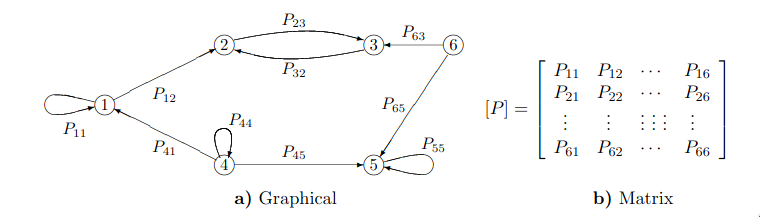
\includegraphics[width=0.8\textwidth]{assets/finite_state_markov_chains.png}
  \caption{Finite 6 State Transition Matrix}
  \label{fig:finite_state_markov_chains}
\end{figure}

\begin{lemma}
  Properties of a transition matrix $P$
  \begin{enumerate}
    \item $P_{i,j} \geq 0$ 
    \item $\sum_{j=1}^{\mid \Omega \mid} P_{i,j} = \sum_{j \in \Omega} P[X_1 = j \mid  X_0 = i] = P[\cup_{j \in \Omega} \{X_1 = j\} \mid X_0 = i]  = 1$
  \end{enumerate}
  This is known as a \textbf{row-stochastic matrix}. 
  \begin{prop}
    A matrix is \textbf{row stochastic} $\iff$ there is a finite state markov chain associated with it $\iff$ there is a weighted directed graph where the weights of outgoing edges from each node sum to 1 (the matrix is the adajency matrix)
  \end{prop}
\end{lemma}

\begin{note}{Example} 
  Consider $P = \begin{pmatrix}
0.2 & 0.5 & 0.3 \\
0.6 & 0.3 & 0.1 \\
0.4 & 0.4 & 0.2
\end{pmatrix}$.
\begin{enumerate}
  \item What is $P(F_0 = 1, F_1 = 2, F_2 = 3, F_3 = 1, F_4 = 1)$ ?

\begin{align*}
P(F_0 = 1, F_1 = 2, F_2 = 3, F_3 = 1, F_4 = 1) 
&= P(F_0 = 1) \cdot P(F_1 = 2 \mid F_0 = 1) \cdot P(F_2 = 3 \mid F_1 = 2) \\
&\quad \cdot P(F_3 = 1 \mid F_2 = 3) \cdot P(F_4 = 1 \mid F_3 = 1) \\
&= 1 \cdot P_{1,2} \cdot P_{2,3} \cdot P_{3,1} \cdot P_{1,1} \\
&= 1 \cdot 0.5 \cdot 0.1 \cdot 0.4 \cdot 0.2 \\
&= 0.004.
\end{align*} 

\item What is $P[F_2 =3|F_0 = 1]$?

\begin{align*}
P(F_2 = 3 \mid F_0 = 1) 
&= \sum_{k=1}^{3} P(F_2 = 3 \mid F_1 = k, F_0 = 1) \cdot P(F_1 = k \mid F_0 = 1) \\
&= \sum_{k=1}^{3} P(F_2 = 3 \mid F_1 = k) \cdot P(F_1 = k \mid F_0 = 1) \\
&= P(F_2 = 3 \mid F_1 = 1) \cdot P(F_1 = 1 \mid F_0 = 1) \\
&\quad + P(F_2 = 3 \mid F_1 = 2) \cdot P(F_1 = 2 \mid F_0 = 1) \\
&\quad + P(F_2 = 3 \mid F_1 = 3) \cdot P(F_1 = 3 \mid F_0 = 1) \\
&= (0.3 \cdot 0.2) + (0.1 \cdot 0.5) + (0.2 \cdot 0.3) \\
&= 0.06 + 0.05 + 0.06 \\
&= 0.17.
\end{align*}
Notice that, $\sum_{k=1}^{3} P(F_2 = 3 \mid F_1 = k) \cdot P(F_1 = k \mid F_0 = 1) = \sum_{k=1}^{3} P_{k,3} \cdot P_{1,k} = (P^{2})_{1,3}$!
\end{enumerate}
\begin{remark}
      Notice that for these finite state markov chains, it is simplest to compute joint probabilities!
\end{remark}
\end{note}

\begin{definition}
  Let $P$ be the transition matrix of a time-homogeneous Markov chain with $m$ states. The $(i,j)$-th entry of $P^n$, denoted $(P^n)_{i,j}$, represents the probability of transitioning from state $i$ to state $j$ in $n$ steps. Formally,

\[
(P^n)_{i,j} = P(F_n = j \mid F_0 = i)
\]

This can be expressed as:

\[
(P^n)_{i,j} = \sum_{k_1=1}^{m} \sum_{k_2=1}^{m} \dots \sum_{k_{n-1}=1}^{m} P_{i,k_1} P_{k_1,k_2} \dots P_{k_{n-1},j}
\]

where the summation is taken over all possible intermediate states $k_1, k_2, \dots, k_{n-1}$.
\end{definition}
\begin{lemma}
  
Let $\alpha = (\alpha_1, \alpha_2, \dots, \alpha_m)$ be the initial distribution, where $\alpha_i = P(F_0 = i)$ for $i = 1, \dots, m$. Then the probability that the chain is in state $j$ after $n$ steps is given by:

\[
P(F_n = j) = (\alpha P^n)_j = \sum_{i=1}^{m} \alpha_i (P^n)_{i,j}
\]
\begin{note}
  We are conditioning over $F_0$
\end{note}

In this case, $\alpha P^n$ is the row vector obtained by multiplying the initial distribution $\alpha$ by the matrix $P^n$. The $j$-th entry of this vector gives the probability that the chain is in state $j$ at time $n$.
\end{lemma}

\subsection{Recurrent States and Absorbing Markov Chains}

\begin{definition}
  A state is  called \textbf{recurrent} if $$P[X_n= i \text{ for infinitely many n's} | X_0 = i] = 1$$. Otherwise, a state is \textbf{transient}.  
\end{definition}
\begin{definition}
  A state is called \textbf{absorbing} if $P_{i,i} = 1$. Every absorbing state is recurrent.
\end{definition}
\begin{definition}
  A markov chain is called absorbing if $\exists $ at least one absorbing state and it is possible to reach an absorbing state from every non-absorbing state (not necessarily in one step). \\

  Mathematically, let $A \subseteq \Omega: A = \{i : P_{ii}=1\} $, the set of absorbing states. We say a chain is abosrbing if:
  \[
  A \neq \emptyset
  .\] 
  and 
  \[
    \forall j \in \Omega \setminus A, \exists a \in A \text{ such that } P[X_n = a | X_0 = j] > 0
  .\] 
  Basically, regardless of intial conditions, there is a positive probability that you will eventually reach an absorping state.  
\end{definition}

\begin{remark}
  Question: Suppose I start at a transient state $j$, what is the probability  $P[$ I get absorbed evenutally  $\mid X_0 \neq j]$?

  \begin{proof}
    Let $i,j$ be transient states in $\Omega$. 
   \begin{align*}
     P[X_n = j \mid X_0 = i] &= P[X_n = j \text{ and $X_k$ is transient  $\forall k \in \{1,2,3, \ldots,n\}$} \mid X_0 = i] \\
                             &\text{ because we know that any intermediate states between $X_n$ and  $X_0$ can't be absorbing} 
   .\end{align*} 
   We can manipulate the transition matrix to have a block structure by permuting the matrix (relabeling nodes):
   \[
     P = \begin{pmatrix} Q & R \\ 0 & I \end{pmatrix}
   .\]  
   where $Q$ are the transient states, $R $ are the connections from the transient to absorbing states, and  $I$ the absorbing states.  For example, the matrix:
\[
P = \begin{bmatrix}
\begin{array}{cc|cc}
0.5 & 0.5 & 0 & 0 \\
0.2 & 0.3 & 0.5 & 0 \\
\hline
0 & 0 & 1 & 0 \\
0 & 0 & 0 & 1
\end{array}
\end{bmatrix}
\]
Then, we can consider
\begin{align*}
  (P^{n})_{i,j} &= P[X_j = j \mid X_0 = i] \\
                &= P[X_n = j \text{ and $X_k$ is transient  $\forall k \in \{1,2,3, \ldots,n\}$} \mid X_0 = i] \\
                &= (Q^{n})_{i,j}
.\end{align*}
  \end{proof}
\end{remark}

\begin{theorem}
  if $P$ represents an absorbing markov chain, then  $Q^{n} \to 0$ the zero matrix. Thus, for any state,
  $P[\text{ eventual absorption} \mid X_0=i] = 1$

  \begin{proof}
    for every transient state $j$,  $\exists m_j$ such that $P[X_{m_j} \in A \mid  X_0 = j] = P_j > 0$. We know 
    \begin{enumerate}
      \item $m = max_{j \in \Omega \setminus A} m_j \leq \infty$ since finite number of states, so finite number of possible steps ($m_j$ represents the  $m_j$th step)
      \item $p = min_{j \in \Omega \setminus A} P_j > 0$ the minimum probability to reach an absorbing state from any starting state
    \end{enumerate}
    Then for $j \in \Omega \setminus A$, $$P[\text{ being absorbed by the m} \mid X_0 = j] \geq p$$. Let $NA(k) = \{\text{the markov chain has not been absorbed within the first k $\cdot$ m steps}\} $. To prove the thorem, it sufficies to show that for any transient state $i$,
     \[
       P[NA(k) \mid X_0 = i] \to 0, k \to \infty
    .\] 
    We will prove the stronger statement by induction
    \[
      P[NA(k) \mid  X_0 = i] \leq (1-p)^{k}
    .\] 
    \begin{enumerate}
      \item Base Case: $P[NA(1) \mid  X_0 = i] \leq (1-p)$ which must be true since $P[NA(1) \mid X_0 =i] = 1 - P[\text{ being absorbed by the m} \mid X_0 = j]  \leq 1 - p$
      \item Induction Step: Assume $P[NA(k) \mid  X_0 = i] \leq (1-p)^{k}$ for any state $i$. 
        \begin{align*}
          P[NA(k+1) \mid  X_0 + i] &= P[NA(k+1) \cap NA(k) \mid X_0 = i] \\
                                   &= P[NA(k) \mid X_0 = i] \cdot P[NA(k+1) \mid NA(k), X_0 =i] \\
                                   &\leq (1-p)^{k} \cdot P[NA(k+1) \mid  NA(k), X_0 = i]\\
                                   &=  (1-p)^{k} \cdot \sum_{j \in \Omega \setminus A} P[NA(k+1) \mid X_{km} = j, NA(k), X_0 = i] \cdot \\ 
                                   &P[X_{km} = j \mid NA(k), X_0=j] \\
                                   &\text{ use markov property}\\
                                   &= (1-p)^{k} \cdot \sum_{j \in \Omega \setminus A} P[NA(k+1) \mid X_{km} = j] \cdot P[X_{km} = j \mid NA(k), X_0=j] \\ 
                                   &\text{ then let's reset the time by setting $km$ to new time  $0$}\\
                                   &= (1-p)^{k} \cdot \sum_{j \in \Omega \setminus A} P[NA(1) \mid X_{0} = j] \cdot P[X_{km} = j \mid NA(k), X_0=j] \\ 
                                   &\leq (1-p)^{k} \cdot (1-p) \cdot \sum_{j \in \Omega \setminus A} P[X_{km} = j \mid NA(k), X_0=j] \\ 
                                   &\text{ if we haven't been absorbed and we go from every possible transient to every other transient, the probabilities sum to 1!} \\
                                   &\leq (1-p)^{k} \cdot (1-p) \cdot 1 \\
                                   &\leq (-1p)^{k+1}
        .\end{align*}
    \end{enumerate}
  \end{proof}
\end{theorem}

\begin{remark}
  How long does it take to get absorbed? What is:
  \[
    E[T \mid X_0 =i] = ?
  .\] 
\end{remark}

\begin{prop}
  If $P$ is an absorbing markov chain with transient block matrix  $Q$, then  $N=(I-Q)^{-1}$ is equal to $I+Q+Q^{2}+Q^{3} + \ldots$ 

  \begin{proof}
    Recall $Ax = 0$ has only the trivial solution  $x=0$ then  $A$ is invertible. This is because  $A$ has full rank and the null space is trivial. So  $(I-Q)x =0$ only when  $x=0$. Then,
     \begin{align*}
       (I-Q)x = 0 &\iff x - Qx = 0\\
                  &\iff x = Qx \\
                  &\iff x = Qx = Q^{2}x = Q^{3}x = \ldots = Q^{n}x 
    .\end{align*}
    Then since $Q^{n} \to 0$ :
    \[
    X = \lim_{n \to \infty} Q^{n} x = 0
    .\] 
    Let $S_{m} = I + Q + \ldots + Q^{m}$.
    \begin{align*}
      (I-Q) \cdot S_m &= (I + Q + Q^{2} + \ldots + Q^{m}) - (Q + Q^{2} + \ldots + Q^{m+1}) \\
                      &= I - Q^{m+1}  
    .\end{align*}
    Take the limit $m \to \infty$, so:
     \begin{align*}
       (I-Q) S_\infty &= \lim_{m \to \infty} I - Q^{m+1} \\
       &= I  
    .\end{align*}
    Since inverses are unique:
    $N = (I-Q)^{-1} = S_\infty$
  \end{proof}
\end{prop}

\begin{prop}
  Let $V(j)$ = number times markov chain visits state  $j$. Then,
   \[
     (N)_{i,j} = E[V(j) \mid  X_0 = i]
  .\] 
  The entries in the inverse of $I-Q$ gives the expected number of times a markov chain starting from $i$ visits  $j$ over an infinite number of steps
  \begin{proof}
    Express $V(j)$ as sum of indicators.
     \[
    M_j^{n} = \begin{cases}
      1, x_n =j \\
      0, x_n \neq =j
    \end{cases}
    .\]
    Using linearity,
    \begin{align*}
      E[V(j) \mid  X_0 = i] &= E[\sum_{n=0}^{\infty} M_j^{n} \mid X_0 =i] \\
                            &= \sum_{n=0}^{\infty} E[M_j^{n}\mid X_0=i]  \\
                            &= \sum_{n=0}^{\infty}  P[X_n = j \mid  X_0 = i] \\
                            &= \sum_{n=0}^{\infty} (Q^{n})_{i,j} \\
                            &= (I + Q + Q^{2} + \ldots) \\
                            &= N_{i,j}
    .\end{align*}
  \end{proof}
\end{prop}

\begin{theorem}
  The expected value of the number of steps until it is absorbed from state $i$ is:
   \[
     E[T \mid  X_0 = i] = E[\sum_{j \in \Omega \setminus A} V(j) \mid  X_0 = i] = \text{ sum of row $i$ in  $N$} 
  .\] 
\end{theorem}

\end{document}
